\documentclass[xcolor=dvipsnames]{beamer}

\usepackage[utf8]{inputenc}
\definecolor{dgreen}{rgb}{0.,0.6,0.}
\definecolor{gold}{rgb}{1.,0.84,0.}

\usepackage{epsfig}
\usepackage{amssymb}
\usepackage{amsmath}
\usepackage{amsfonts}



\title{Cooling-Aware Geographical Load Balancing Visualized}

\subtitle{Research supported by NSF, Elliot Family, and Rose Hills Foundation}

\author[Hirshleifer, Wang, Liu, Wierman] % (optional, for multiple authors)
{Michael~Hirshleifer\inst{} \and Yizhen~Wang\inst{} \\ \and Zhenhua~Liu \inst{} \and Adam~ Wierman \inst{}}
\institute[Caltech] % (optional)
{
  \inst{}%
  California Institute of Technology \\
  1200 E California Blvd \\
   Pasadena, CA 91106 \\
 % \and
 % \inst{2}%
  %Institut für theoretische Philosophie\\
  %Universität Dort
}
\date[Support] % (optional)
{Caltech SURF Presentation, October 2012 }
%\subject{Informatik}


% TOC at start of each section
\AtBeginSection[]
{
  \begin{frame}
    \frametitle{Table of Contents}
    \tableofcontents[currentsection]
  \end{frame}
}


\newcommand{\carbondioxide}{\ensuremath{\mathrm{CO}_2}}
\newcommand{\eqdef}{\ensuremath{\overset{\mathrm{def}}{=}}}



% \author{
% % You can go ahead and credit any number of authors here,
% % e.g. one 'row of three' or two rows (consisting of one row of three
% % and a second row of one, two or three).
% %
% % The command \alignauthor (no curly braces needed) should
% % precede each author name, affiliation/snail-mail address and
% % e-mail address. Additionally, tag each line of
% % affiliation/address with \affaddr, and tag the
% % e-mail address with \email.
% %
% % 1st. author
% \alignauthor
% Michael Hirshleifer\\
% 	\affaddr{California Institute of Technology}\\
% 	\affaddr{1200 E California Blvd}\\
% 	\affaddr{Pasadena, California}\\
% 	\email{111mth@caltech.edu}
% % 2nd. author
% \alignauthor
% Yizhen Wang\\
% 	\affaddr{California Institute of Technology}\\
% 	\affaddr{1200 E California Blvd}\\
% 	\affaddr{Pasadena, California}\\
% 	\email{ywang3@caltech.edu}
% \and
% % 3rd. author
% \alignauthor
% Zhenhua Liu\\
% 	\affaddr{California Institute of Technology}\\
% 	\affaddr{1200 E California Blvd}\\
% 	\affaddr{Pasadena, California}\\
% 	\email{zliu2@caltech.edu}
% % the prof
% \alignauthor
% Adam Wierman\\
% 	\affaddr{California Institute of Technology}\\
% 	\affaddr{1200 E California Blvd}\\
% 	\affaddr{Pasadena, California}\\
% 	\email{adamw@caltech.edu}
% }
% 
% \date{2012-10-02}

\begin{document}

\frame{\titlepage}

\begin{frame}
\frametitle{Outline}
\tableofcontents[part=1,pausesections]
\end{frame}

\begin{frame}{Summary}

	\begin{block}{Research Goal}  
	Develop software to show how geographical load balancing (GLB) improves data center (DC) efficiency use of renewable energy.  
	\end{block}
	
	\begin{block}{Issue} 
	Minimize DC electricity cost over time by convex optimization over real workload inputs - temp, solar, \& wind traces.
	\end{block}

	\begin{block}{Our Contributions} 
	\begin{itemize}
		\item{Cooling-aware GLB model \\
			DCs use locally available renewable energy more effectively \\
			Reduce electricity grid usage, even across seasons \\
			Potentially use renewables almost exclusively} 
		\item{Visualization \\ 
		Animation of 10 DCs demand \& energy usage (grid \& renewable energy generation) in 48 contiguous U.S. states}  
		\item{Test effectiveness of, and refine, routing algorithms using visualization}
	\end{itemize} 
	\end{block}

\end{frame}

\section{Introduction}

\begin{frame}{Background}

	\begin{block}{Strong need for “green” routing algorithms to reduce electricity costs and pollution} 
		Many, high growth in DC; DC energy usage major source of operating costs; DCs consume high fraction of US/world non-green energy production; Major polluter.
	\end{block}

	\begin{block}{DC servers energy use} \vspace{-1mm}
		\begin{itemize}
		          \item{To operate and \textbf{cool} (previously ignored in literature)}
			\item{Substantial and variable (especially for cooling in summer). \\ %\cite{datacenter} 
				\begin{itemize} \item{Exploit geog.heterogeneity of DC cooling costs.) } \end{itemize}
				}
			\item{Some DCs partly operated on green energy (solar, wind); Problem - green energy highly variable 
				\begin{itemize} \item{Time of day, cloud cover, wind speed.}
					               \item{Does not match user demand. }
				\end{itemize} }
			\item{Prohibitively expensive to store green energy.}
			\item{Need to buy off of grid, increase pollution.}
		\end{itemize}
	\end{block}

\end{frame}

\begin{frame}{Previous GLB models}

	\begin{block}{Old models}
		Solve DC redundancy by geographical routing to minimize latency; Ignore energy efficiency.
	\end{block}

	\begin{block}{Wierman group's green GLB model, Liu et al 2011 } % \cite{adam:GLB}
		\begin{itemize}
			\item{Tradeoffs min. latency from geographical distance and min. electricity costs using green sources.}
			\item{Optimal or near-optimal  routing algorithms for efficient GLB (given functional form for cost of increased latency).}
			\item{Can power DC networks almost entirely off renewable energy without undue increase in latency} 
		\end{itemize}
	\end{block}  	
\end{frame}

\begin{frame}{Cooling-aware geographical load balancing model}

%	\begin{block}{Contributions}
		\begin{itemize}
			\item{Consider cooling costs.} 
			\item{Solution achieves significantly lower total energy cost \& lower \carbondioxide{} emission.}
			\item{Evaluate economic, environmental impact.}
			\item{Use actual data center workload, weather, renewable energy (wind, solar) availability and grid electricity prices to numerically compute the optimal solution.}
			\item{10 Data Center locations in 48 contiguous U.S. states.} 
			\item{Implement visualization of simulation solution \\
				Advantages: 
				\begin{enumerate}
					\item{Easier to see what each optimization algorithm is doing.}
					\item{Can test effectiveness of, and refine, routing algorithms.} 
					\item{Facilitate development of an implementable algorithm.}
				\end{enumerate}
				}			
		\end{itemize}
%	\end{block}
\end{frame}

\begin{frame}{Cooling-aware GLB model results}

	\begin{block}{Low variation in optimized cost despite volatile wind, sun.}
		\begin{itemize} 
			\item{Solution reduces total system cost by distributing requests to locations with cheap energy, favorable weather for cooling.}
			\item{Addresses DC cooling in locations with extreme climate or weather (diurnal temp. variation).}
		\end{itemize}
	\end{block}
	\vspace{-3mm}
	\begin{block}{Reduction in \carbondioxide{}, halved}
	\end{block}
	\vspace{-3mm}
	\begin{block}{More comprehensive treatment of energy costs sources - cooling; better-informed decisions.}
	\end{block}
	\vspace{-3mm}
	\begin{block}{Considering cooling superior to adding non-green storage to model lowers total cost and carbon emissions.}
	\end{block}
	\vspace{-3mm}
	\begin{block}{Lower infrastructure investment, easier to implement }
	\end{block}
\end{frame}

\section{Setup}

\begin{frame}{Model Setup}

Each DC has a cooling system. % (\cite{adam:cooling}). 
Modify Liu et al.'s (2011) %\cite{adam:GLB}% 
model to include cooling costs. Use convex optimization to solve model as in Liu et al. (2011b). %\cite{adam:GLBfull}.

	\begin{block}{Workload}

	Web of source requests assumed at geog. centers in 48 U.S. states. 

	$L_j(t)$, mean request arrival rate from source $j$ at interval $t$ from real-world traces.

	Workload base trend from trace at H-P Labs.

	Scale workload of each request source by state population. 

	\end{block}

	\begin{block}{Renewable energy output} 

            Use 10min interval real wind speed \& insolation traces from http://wind.nrel.gov/.  %\cite{renew1} \cite{renew2}. 
	%@@@@@@[Is this true? I thought the traces were (calculated) power output.] 

	\vspace{1mm}
           DC renewable energy generation rate per plant $\propto$   Weather data.

	Total renewable energy =  $c$ $\times$ Total energy demand to process all requests, 	$c$ varies in $[0.5, 4]$ with a step length of $0.5$.

	 Use a mix of 80\% of wind and 20\% following Liu et al. (2011). % \cite{adam:GLB}.
	\end{block}
\end{frame}

\begin{frame}{The internet-scale system}

Set $\mathcal{N}$ of 10 DCs at Google DCs in 10 states. \vspace{1mm}  %California, Washington, Oregon, Illinois, Georgia, Virginia, Texas, Florida, North Carolina, and South Carolina. 

\#servers $X_i$ at DC $i$ = 2 $\times$ peak load at $i$  \vspace{1mm} 

% ***** when all requests are routed to nearest DCs. ******

Optimization: Choose routing plan $\lambda_{ij}(t)$ and \# active servers $x_i(t)$  to minimize total cost (= delay cost + energy cost + switching cost).

\begin{block}{Delay cost}
= Propagation delay $d_{ij}$ from source $j$ to DC$_i$  + queuing delay at $i$.

$d_{ij}$ = travel time from $i$ to $j$ at transmission speed $200 \frac{\mathrm{km}}{\mathrm{ms}}$ + $5 \mathrm{ms}$. \vspace{1mm} 

Queuing delay calculated from the parallel M/G/1/Processor.  \vspace{1mm} 

Sharing queue model: Total load $\lambda_i(t)=\sum_j \lambda_{ij}(t)$ distributed evenly across $x_i(t)$ homogeneous servers of service rate \mbox{$\mu_i$ = $0.1 / \mathrm{ms}$}.

\end{block}

\end{frame}

\begin{frame}{Cooling-aware optimization}

	Minimize energy consumption to maintain DC at $T = 25^{\circ}\textrm{C}$. 

	\#active servers $x = x_a + x_c$  where a=air-cooled, c=water chilled. \vspace{1mm} 

	Find best division between $x_a$ and $x_c$.

	\begin{block}{Air-cooling energy consumption} \vspace{-3mm}
	\begin{equation}
           c_a(x) = k \cdot x^3, 0 \leq x \leq \bar{x}, k > 0
 	\end{equation}

 $k$ $\propto$ temperature gradient between the inside and outside air. 

$\bar{x}$ = maximum \#servers cooled by air cooling alone. 

$\bar{x}$ $\propto$ temperature gradient, maximum air flow rate. 

\vspace{2mm}

We set air flow rate to level that can air cool DC entirely at full workload when outside temperature is lower than   $T - 20^{\circ}\mathrm{C}$. 
\end{block}
\end{frame}

\begin{frame}{Chilled-water cooling}

Energy consumption roughly linear in IT demand empirically: 
\begin{equation}
c_c(x) = \gamma \cdot x
\end{equation}
%Here $\gamma = 0.17$, meaning that the chiller takes 0.17kW/h electricity to cool the heat caused by 1kw/h of IT demand.
%For notational convenience, define
\begin{equation}
	x^+ \eqdef \min(0, x)
\end{equation}
% to be $x$ clamped to be positive.

\begin{block}{Optimal cooling portfolio}
\begin{equation}
c(x) = \min_{x_c \in [0,x]} \gamma \cdot (x-x_c)^+ + kx_2^3
\end{equation}
which yields
$$
c(x) = \left\{ \begin{array}{ll}
	k \cdot x^3 & \mbox{if $x \geq x_s$}\\
	k \cdot x_s^3 + \gamma \cdot (x-x_s) & \mbox{otherwise}\end{array} \right.
$$
where $x_s = \min \left(\sqrt{\gamma/3k}, \bar{x}\right)$ is the threshold for when chiller cooling is necessary.

\end{block}
\end{frame}

%To explore seasonality on cooling model performance
% Hourly temperature data from Week 1 January 2012 from \cite{temp} and Week 1 July 2012. 

\begin{frame}{Data center visualization}

\begin{figure}
\centering
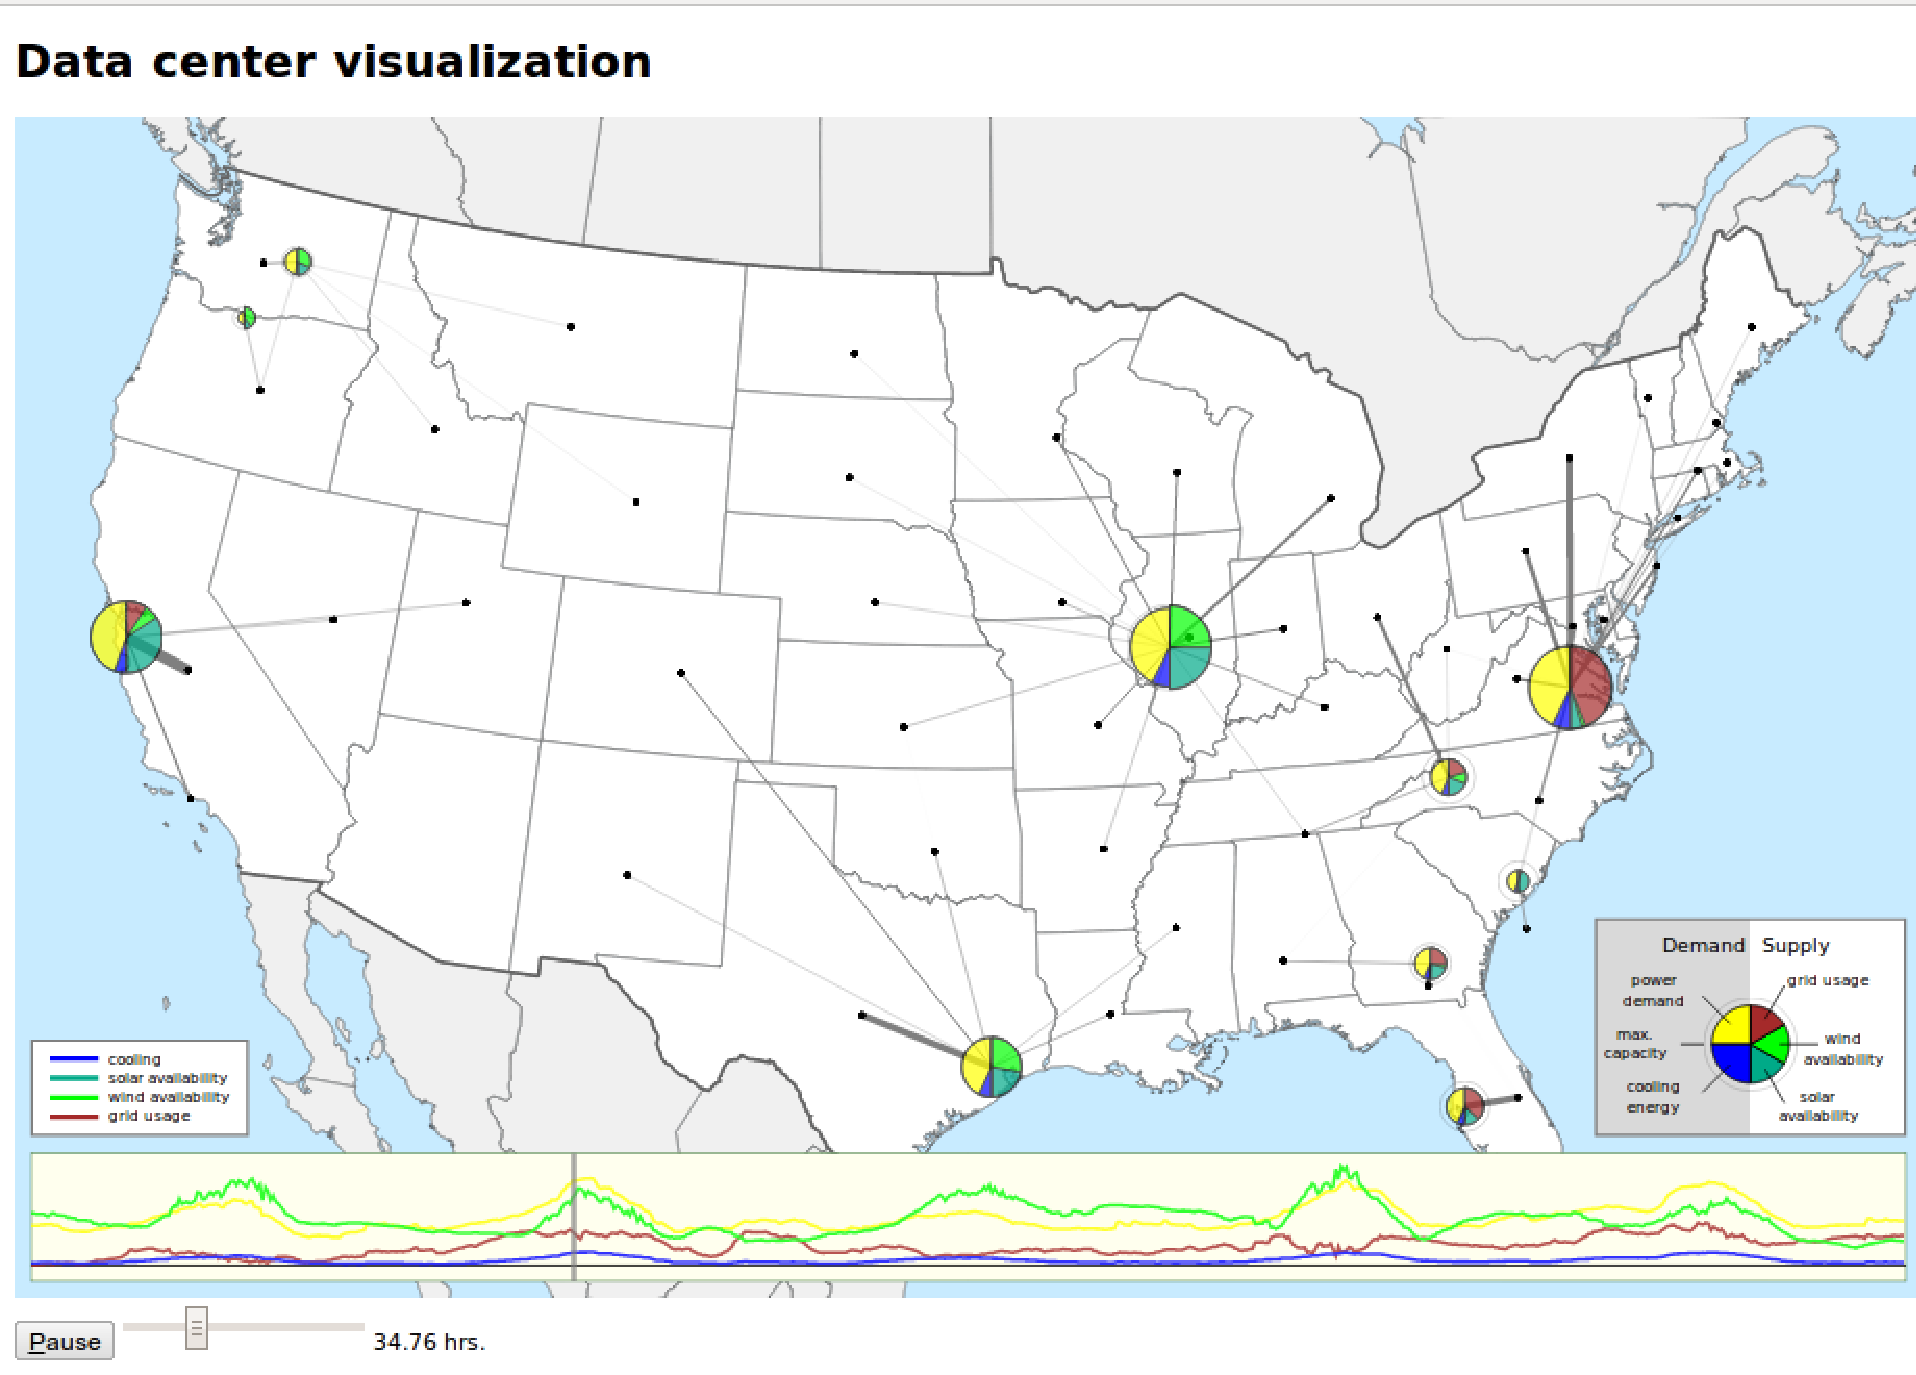
\epsfig{file=visualization-bmp.pdf, height=3in, width=4.5in}
\caption{Screenshot of the visualization, running in the Chromium web browser.}
\end{figure}

\end{frame}

\begin{frame}{}
\begin{block}{Energy cost}
Cost of running active servers + cost of maintaining constant working temperature. 

Assume DC renewable energy cost is 0. 

Grid energy cost: \vspace{-3mm}
\begin{equation}
p_i \cdot (l(x_i(t)) + c(x_i(t)) - r_i(t))^+
\end{equation}
$p_i$ = electricity price, 
$x_i(t)$ = \#active servers in time interval $t$,

$l(x_i(t))$ = linear function of energy consumption, %of active servers or IT demand in time interval 
$c(x_i(t))$ = energy usage for cooling, $r_i(t)$ = renewable energy availability, 

$p_i$  = constant real statistic for each state. 
\end{block}

\begin{block}{Switching cost}
Delay, wear \& tear cost switching on/off servers. DC workload updated every 10 mins. Switching cost weight $\beta = 6$.
$$\beta \cdot (x_i(t+1) - x_i(t))^+$$
\end{block}

\end{frame}

\begin{frame}{}

\begin{block}{Storage}
DC can store energy (batteries, supercapacitors, flywheels).

Electricity storage at time $t$ is $0 \leq es_i(t) \leq ES_i$. 

$ES_i$ = maximum storage capacity.  Storage rate is
$$e_i(t) = \rho \cdot (es_i(t) - es_i(t+1))$$
Positive $e_i(t)$ means discharging, negative charging. 

Assume $\rho = 1$, charging or discharging efficiency is perfect.

Energy cost with storage is
\begin{equation}
p_i \cdot (l(x_i(t)) + c(x_i(t)) - r_i(t) - e_i(t))^+
\end{equation}
\end{block}
\end{frame}

\begin{frame}{Optimization problem - Minimize total costs}

\begin{align*}
\min_{\bf{x}(t), \bf{\lambda}(t)} & \sum_{i \in \mathcal{N}} p_i \cdot (l(x_i(t)) + c(x_i(t)) - r_i(t) - e_i(t))^+ \\
& + \sum_{j \in \mathcal{J}}\sum_{i \in \mathcal{N}}
\lambda_{ij}(t)\left(\frac{1}{\mu_i - \lambda_i(t)/x_i(t)} + d_{ij}\right) \\
& + \beta \cdot (x_i(t+1) - x_i(t))^+
\end{align*}
\vspace{-2mm}
subject to
\begin{align*}
& \sum_{i\in \mathcal{N}}\lambda_{ij}(t) = L_j(t), &\forall j\in J \\
& \lambda_{ij} \geq 0, & \forall i\in N, j\in J \\
& 0 \leq x_i(t) \leq X_i, & \forall i \in N \\
& \lambda_i(t) \leq x_i(t) \cdot \mu_i & \forall i \in N \\
& 0 \leq es_i(t) \leq ES_i & \forall i \in N \\
& e_i(t) = es_i(t) - es_i(t+1) & \forall i \in N
\end{align*}

\end{frame}

\begin{frame}{}

	\begin{block}{Boundary conditions model real-world constraints:}
	\begin{enumerate}
	\item
	GLB system processes all requests. Each DC gets $>0$ work.
	\item
	Each DC has finite server capacity. %cannot process requests $>$ computational capacity; server capacity finite.
	\item
	Each DC's energy storage capacity bounded [$0$, fixed cap].
	\end{enumerate}
	\end{block}
\vspace{-3mm}
\begin{block}{\carbondioxide{} emission}
\vspace{-3mm}
$$\sum_{i \in \mathcal{N}} \eta_i \cdot (x_i(t) + c(x_i(t)) - r_i(t) - e_i(t))^+$$
Emissions rate $\eta_i$ per kW$\cdot{}$h varies across states based on energy-source composition.  %estimates available from \cite{carbon}.
\end{block}

%\end{frame}

%\begin{frame}{}

\begin{block}{Benchmarks to compare Cooling-aware GLB to GLB LOCAL.}
%To show effect of integrating cooling concerns into GLB, 
%For the two benchmark models, the cooling optimization is done after the routing scheme is determined.
Assume 3-hr and 6-hr storage systems, no running costs for storage, finite storage capacity. 
% quantified as duration DC operates at max load entirely off stored energy (excl. cooling usage). 
\end{block}
\begin{block}{Evaluate outcomes based on 1) the total cost, 2) grid (brown) energy usage, 3) \carbondioxide{} emissions.}
\end{block}
\end{frame}

%\begin{frame}{}
%	\begin{figure}
%	\centering
%	\epsfig{file=cost_comparison.pdf, height=1.8in, width=7in}
%	\caption{Comparison of optimal costs of Cooling-aware GLB, Cooling-oblivious GLB and LOCAL, with varying renewable energy availability.}
%	\end{figure}
%\end{frame}

\begin{frame}{}
	\begin{figure}
	\centering
	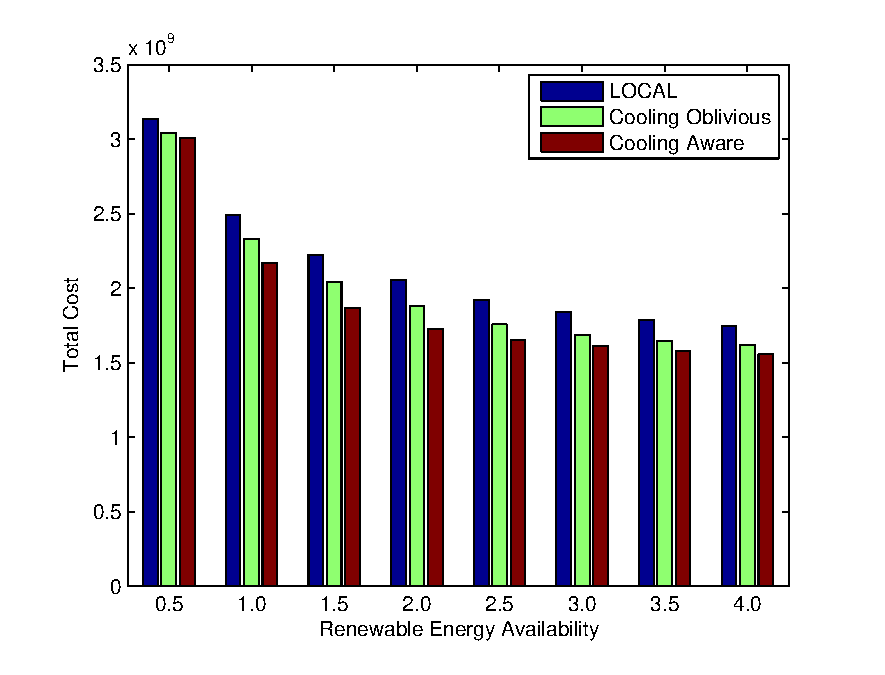
\epsfig{file=cost_summer.pdf, height=1.8in, width=4.2in}
	\caption{Summer optimized costs of Cooling-aware GLB, Cooling-oblivious GLB and LOCAL, with varying renewable energy availability.}
	\end{figure}
\end{frame}

\begin{frame}{}
	\begin{figure}
	\centering
	\epsfig{file=cost_winter.pdf, height=1.8in, width=4.2in}
	\caption{Winter optimized costs of Cooling-aware GLB, Cooling-oblivious GLB and LOCAL, with varying renewable energy availability.}
	\end{figure}
\end{frame}

\section{Visualization}
\begin{frame}{Motivation for Visualization}
Numerical simulation result is very large time series describing routing plans and data center activity. \\
\vspace{2mm}
Hard to interpret large quantity of data in matrix form. \\
\vspace{2mm}
Visualization:  
	\begin{itemize}
	\item Key characteristics of the optimal solution salient.
	\item Acts as simple check for validity of solution
	\item An obvious way to spot abnormal behaviors in the output.
	\end{itemize}
\end{frame}
\begin{frame}{Technical description}
 	\begin{block}{Scalable Vector Graphics (SVG) format}
	High-quality XML-based vector graphics format supports fluid animations displaying time-series data. \\ 
	Animation can be embedded into a web page.
	\begin{block}{Wrapper XHTML web page} 
	Implemented using Javascript \\	
	User-friendly, can control animation (play, pause, or seek) using web interface \\
	Possible enhancements could include zooming, panning, and showing/hiding types of map elements.
	\begin{block}{Both components work in the Chromium web browser and pass the W3C validators}
	\end{block}
	\end{block}
	\end{block}
\end{frame}
\begin{frame}{Technical description, contd.}
	\begin{block}{Back-end script generating SVG map from input data}
	Written in Scala programming language. \\
	Script reads in and displays DC center locations, client (request source) locations, real solar- and wind-generation traces. \\
	Routings optimized using various algorithms (from Matlab optimization outputs). \\
	Raw input data in CSV format.\\
	Matlab outputs exported to NetCDF format for reading into Scala.
	\end{block}
	\begin{block}{Background map of the 48 contiguous United States}
		\begin{itemize} 
		%Obtained from Wikimedia Commons. \\
	\item 	Points on map correspond to real-world $(latitude, longitude)$ coordinates according to a mathematical transformation specified with map. 
	\item 	Allows drawing physical locations at correct positions on map.
		\end{itemize}
	\end{block}
\end{frame}

\begin{frame}{Graphical representation details}

	\begin{block}{Visualization's three components}
	Animation of dynamic status of the GLB system. \\
	Line plot of aggregate statistics of energy supply and demand. \\  
	Progress bar allows progress scroll and control.
	\end{block}

	\begin{block}{Features}
	Animation displays 10 data centers on base map of United States. \\
	Sector diagram represents each DC's status, which is animated over time. \\
	Circle's left half is DC's energy demand: 
		\begin{itemize}
		\item{\textcolor{gold}{Yellow sector = energy demand for processing the request}}
		\item{\textcolor{blue}{Blue sector = energy demand for cooling} }
		\end{itemize}
	Circle's right half is energy supply: 
		\begin{itemize}
		\item{\textcolor{green}{Light green sector = available wind energy}}
		\item{\textcolor{dgreen}{Dark green sector = available solar energy}}
		\item{\textcolor{brown}{Brown sector = energy usage from the grid}}
		\end{itemize} 
           \end{block} 
\end{frame}

\begin{frame}{Graphical representation details, contd.}

	Area of sector $\propto$ amount of energy (so radius $\propto$ to $\sqrt{}$). \\ 
	Faint circle surrounding sector diagram represents maximum energy usage when DC operates at full load. \\
	Request traffic $\lambda_{d,s}(t)$ represented by lines connecting each source $s$ and destination data center $d$. 
	Line width linearly $\propto$ $L_s(t)$, total volume of requests from $s$. \\
	Line transparency linearly $\propto$ ${\lambda_{d,s}(t)} / {L_s(t)}$, percentage of traffic from source $s$ routed to DC.  \\
	Solid black line means all requests from $s$ are sent to $d$. \\
	Fully transparent line means no traffic routed from $s$ to $d$.
	Line plot displays four aggregate statistics of interest over time: 
	\begin{itemize}
	\item{\textcolor{gold}{Yellow line = aggregate IT power}}
	\item{\textcolor{blue}{Blue line = aggregate energy usage on cooling}}
	\item{\textcolor{green}{Light green line = aggregate wind energy available}}
	\item{\textcolor{dgreen}{Dark green line = aggregate solar energy available}.}
	\end{itemize}
	Bottom progress indicates time elapsed in animation. \\
	User can pause/resume animation and seek to desired time.

\end{frame}

\section{Test effectiveness results}

\end{document}

\begin{frame}{Cost savings from Cooling-aware GLB}

\begin{figure}
\centering
\epsfig{file=cost_diff.pdf, height=2.2in, width=3.2in}
\caption{The difference between optimal costs in summer/winter for both Cooling-aware and Cooling-oblivious GLB}
\end{figure}

The cooling-aware geographical load balancing model reduces firm's energy cost by routing the requests to locations where energy is cheap and cooling is easy. Such a savings outweighs the increase in delay cost. Hence our model is consistent profit maximization by a firm.

%In this experiment, the aggregate amount of renewable energy is set to be the total IT demand multiplied by a coefficient, where the coefficient series is the integer multiples of 0.5 within [0.5, 4]. We run the experiment under both summer and winter weather.

Our first experiment explores the cost efficiency of the this model. Figure 2 illustrates the extent of total cost savings of our model. We choose the total cost under Cooling-oblivious GLB and LOCAL as the benchmark. The Cooling-aware model gives lower cost than both benchmarks. This edge is rather clear under two situations. First, in summer when cooling is expensive, the Cooling-aware model significantly outperforms Cooling-oblivious model; by considering the energy cost of cooling, it makes routing decisions to use renewable energy optimally. Second, when the aggregate renewable energy available lies between once and twice the aggregate demand, and some but not all data center locations have a surplus in renewables, the Cooling-aware GLB exploits this surplus better than the benchmarks.

We are interested in how well the Cooling-aware GLB model works in different seasons and weather conditions. Figure 3 shows the difference between the optimized costs in summer and in winter using each model. The previous Cooling-oblivious model's performance varies significantly with seasonality; our Cooling-aware GLB model's performance is more robust. This finding suggests that our Cooling-aware model exploits the heterogeneity in weather to reduce the energy required for cooling.
%\begin{figure}
%\centering
%\epsfig{file=opt_cost_comparison.pdf, height=2.2in, width=3.2in}
%\caption{A sample black and white graphic (.eps format).}
%\end{figure}
\end{frame}


\begin{frame}{Environmental impact - \carbondioxide{} savings}


\begin{figure}
\centering
\epsfig{file=carbon_summer.pdf, height=2.2in, width=3.2in}
\caption{Comparison of carbon emission of Cooling-aware GLB, Cooling-oblivious GLB and LOCAL.}
\end{figure}


The geographical load balancing method model exploits variation in energy costs by routing requests to where energy cost is low. When the data centers have on-site renewable energy plants (as in our setting), renewable energy becomes cheap; the model allows optimal usage of these renewables and thus has the desirable side-effect of reducing carbon emissions.

We can estimate the \carbondioxide{} emissions by multiplying the grid energy usage of each data center location by the \carbondioxide{} emission per energy unit. Figure 4 shows the \carbondioxide{} emission comparison of each model in summer. By using the Cooling-aware GLB model, aggregate carbon emissions can be reduced by more than 50\% as compared to LOCAL if the total renewable energy supply is equal to the total IT demand. If more renewable energy is available, the carbon emission of Cooling-aware GLB is even less than half of that of Cooling-oblivious GLB.

The environmental impact of our new model is significant. \carbondioxide{} emissions are reduced even even when firms' optimizations do not consider the environmental externality of \carbondioxide{} emissions. Environmental benefits could be even greater if firms are given incentives to be environmentally friendly.
\end{frame}

\begin{frame}{GLB versus Storage}

\begin{figure}
\centering
\epsfig{file=cost_storage.pdf, height=2.2in, width=3.2in}
\caption{Comparison of optimal costs of the storage model and the Cooling-aware GLB model.}
\end{figure}
\begin{figure}
\centering
\epsfig{file=brown_storage.pdf, height=2.2in, width=3.2in}
\caption{Comparison of brown energy usage of the storage model and the Cooling-aware GLB model.}
\end{figure}
One alternative way of using renewable energy efficiently is to store the extra renewables at some moments for future use. Whereas applying geographical load balancing adjusts energy demand according to supply in each location, adding energy storage adjusts supply according to demand. We are interested in the performance characteristics of both methods. In this experiment, we compare the cost curve and the brown energy usage curve of using GLB and using storage. Since our experiment starts at midnight, the time when the data centers are likely to have used all of its storage for batch jobs \cite{adam:cooling}, we assume that the storage starts empty.

Figure 5 illustrates the trend of optimal costs of these models with respect to varying renewable availability. It shows that Cooling-aware GLB has lower costs when the total renewable energy is less than 1.5 times the aggregate IT demand, and the storage model is better when renewable energy is in large surplus.

Figure 6 compares brown energy under each model. The result suggests that the Cooling-aware GLB model needs less energy from the grid compared to the 6-hour-storage curve when the total renewable supply is less than 1.5 times of the total IT power demand. Moreover, it needs less grid energy than the total renewable energy compared to the 3-hour-storage model, in almost the entire renewable availability interval, except when the renewable availability coefficient is 0.5. The environmental impact advantage of our new model is even more salient than to the cost advantage.

We thus can conclude that our model is better than the storage model when the renewable generation facilities are not yet built, because it requires less prior infrastructure investment.
\end{frame}

\section{Future work}
\begin{frame}{Future work}
Our simulation and visualization software can be used to answer questions about extensions to the model that would be useful when putting it into practice, such as—
\begin{itemize}
\item incorporating other kinds of renewables into the model
\item treating data centers as endogenous. In the long run, where should we build new data centers, and what local renewables and energy storage systems do we use?
\item finding the optimal control timescale. It is costly to switch servers on and off, so the current algorithms only change routing every fixed period, which is suboptimal. This significantly restricts the savings that follow-the-renewables routing can yield, but the topic hasn’t yet been explored deeply. Being able to simulate the whole system helps for this.
\item helping discover and then exploit emergent phenomena when looking at systems of many data centers. An example of such a phenomenon deals with the optimal mix of renewable energy for powering data centers. Since the sun shines in the daytime when people are awake and searching the internet, one might expect solar power to dominate. But Wierman’s paper showed that in fact wind is more effective, because its low spatial and temporal correlation is especially useful for geographical load balancing. With solar power, when requests come at night you are forced to buy electricity off the grid, but with wind power, it’s almost always windy somewhere.
\end{itemize}

\end{frame}

\end{document}
